% https://imathworks.com/tex/tex-latex-drawing-a-chord-net-with-tikz/

\documentclass{standalone}

\usepackage{tikz}
\usepackage{pgfplots}
\usetikzlibrary{fillbetween}

\begin{document}

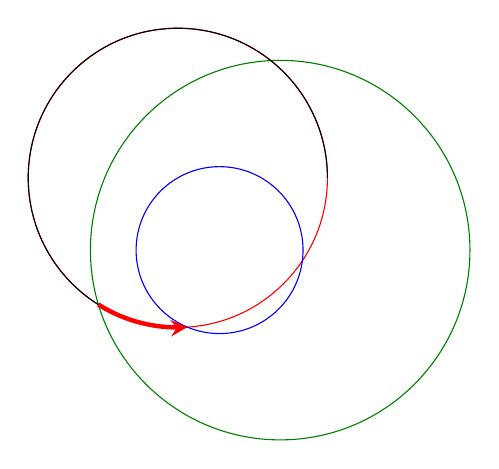
\begin{tikzpicture}

\draw [name path=red,red] (120:1.06) circle (1.9);
%\draw [name path=yellow,yellow] (0:1.06) circle (2.12);
\draw [name path=green,green!50!black] (0:0.77) circle (2.41);
\draw [name path=blue,blue] (0:0) circle (1.06);

% substitute this temp path by `\path` to make it invisible:
\draw[name path=temp1, intersection segments={of=red and blue,sequence=L1}];
\draw[red,-stealth,ultra thick, intersection segments={of=temp1 and green,sequence=L3}];

\end{tikzpicture}

\end{document}